\documentclass[11pt]{article}
\usepackage[utf8]{inputenc}
\usepackage[table]{xcolor}
\usepackage[table]{xcolor}
\usepackage{amsmath,amsthm,amsfonts, amssymb,hyperref,array,xcolor,multicol,
	verbatim,enumitem}
\usepackage[T1]{fontenc}
\usepackage{tikz}
\usetikzlibrary{positioning}
\usetikzlibrary{arrows,decorations.markings}

\begin{document}

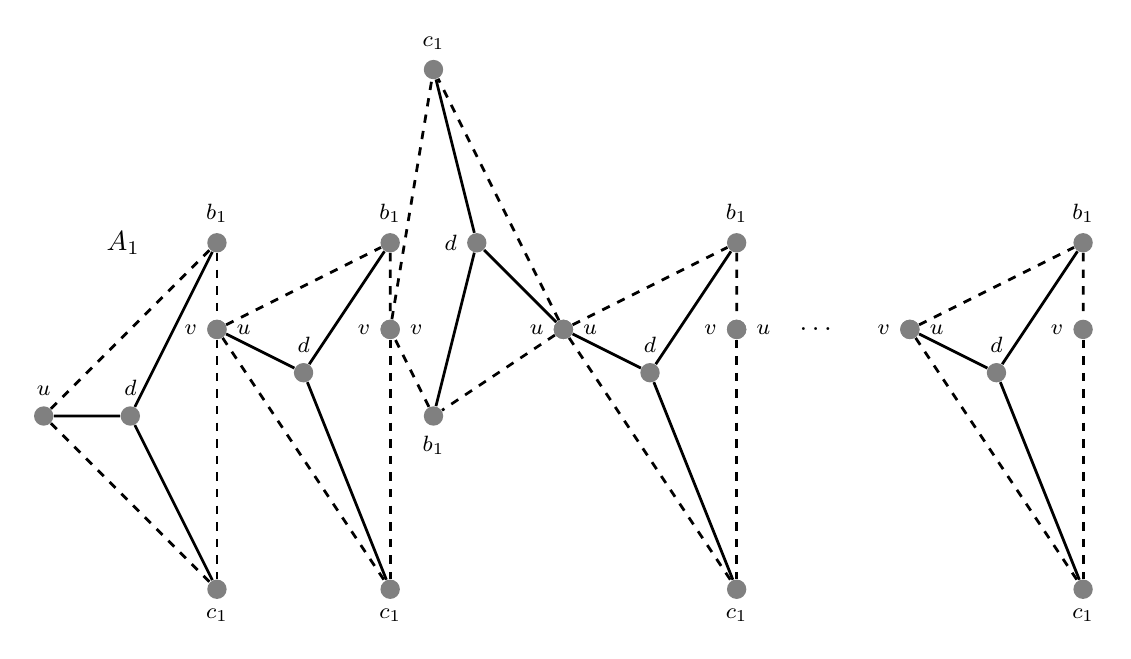
\begin{tikzpicture}[scale=0.55] %shorten >=1pt,->
		
		\tikzstyle{vertex}=[circle,fill=black!50,minimum size=7pt,inner sep=0pt]

        \node[label=right:{$A_1$}] (M1) at (-3,8) {};
        \node[vertex, label=above:{\footnotesize{$b_1$}}] (b11) at (0,8) {};
        \node[vertex, label=above:{\footnotesize{$b_1$}}] (b12) at (4,8) {};
        \node[vertex,label=below:{\footnotesize{$b_1$}}] (b13) at (5,4) {};
        \node[vertex,label=above:{\footnotesize{$b_1$}}] (b14) at (12,8) {};
        \node[vertex,label=above:{\footnotesize{$b_1$}}] (b16) at (20,8) {};

        \node[vertex, label=below:{\footnotesize{$c_1$}}] (c11) at (0,0) {};
        \node[vertex, label=below:{\footnotesize{$c_1$}}] (c12) at (4,0) {};
        \node[vertex,label=above:{\footnotesize{$c_1$}}] (c13) at (5,12) {};
        \node[vertex,label=below:{\footnotesize{$c_1$}}] (c14) at (12,0) {};
        \node[vertex,label=below:{\footnotesize{$c_1$}}] (c16) at (20,0) {};

        \node[vertex, label=above:{\footnotesize{$u$}}] (a11) at (-4,4) {};
        \node[vertex, label=right:{\footnotesize{$u$}}] (a12) at (0,6) {};
        \node[vertex,label=left:{\footnotesize{$u$}}] (a13) at (8,6) {};
        \node[vertex,label=right:{\footnotesize{$u$}}] (a14) at (8,6) {};
        \node[vertex,label=right:{\footnotesize{$u$}}] (a15) at (12,6) {};
        \node[vertex,label=right:{\footnotesize{$u$}}] (a16) at (16,6) {};

        \node[vertex, label=above:{\footnotesize{$d$}}] (d1) at (-2,4) {};
        \node[vertex, label=above:{\footnotesize{$d$}}] (d2) at (2,5) {};
        \node[vertex,label=left:{\footnotesize{$d$}}] (d3) at (6,8) {};
        \node[vertex,label=above:{\footnotesize{$d$}}] (d4) at (10,5) {};
        \node[vertex,label=above:{\footnotesize{$d$}}] (d6) at (18,5) {};


        \node[vertex, label=left:{\footnotesize{$v$}}] (v1) at (0,6) {};
        \node[vertex, label=left:{\footnotesize{$v$}}] (v2) at (4,6) {};
        \node[vertex,label=right:{\footnotesize{$v$}}] (v3) at (4,6) {};
        \node[vertex,label=left:{\footnotesize{$v$}}] (v4) at (12,6) {};
        \node[vertex,label=left:{\footnotesize{$v$}}] (v5) at (16,6) {};
        \node[vertex,label=left:{\footnotesize{$v$}}] (v6) at (20,6) {};


        



% Triangles 
        \draw[line width= 1pt,dashed,-] (a11) -- (b11);
        \draw[line width= 1pt,dashed,-] (b11) -- (v1);
        \draw[line width= 1pt,dashed,-] (v1) -- (c11);
        \draw[line width= 1pt,dashed,-] (a11) -- (c11);
        \draw[line width= 1pt,-] (d1) -- (c11);
        \draw[line width= 1pt,-] (d1) -- (b11);
        \draw[line width= 1pt,-] (d1) -- (a11);

        \draw[line width= 1pt,dashed,-] (a12) -- (b12);
        \draw[line width= 1pt,dashed,-] (b12) -- (v2);
        \draw[line width= 1pt,dashed,-] (v2) -- (c12);
        \draw[line width= 1pt,dashed,-] (a12) -- (c12);
        \draw[line width= 1pt,-] (d2) -- (c12);
        \draw[line width= 1pt,-] (d2) -- (b12);
        \draw[line width= 1pt,-] (d2) -- (a12);

        \draw[line width= 1pt,dashed,-] (a13) -- (b13);
        \draw[line width= 1pt,dashed,-] (b13) -- (v3);
        \draw[line width= 1pt,dashed,-] (v3) -- (c13);
        \draw[line width= 1pt,dashed,-] (a13) -- (c13);
        \draw[line width= 1pt,-] (d3) -- (c13);
        \draw[line width= 1pt,-] (d3) -- (b13);
        \draw[line width= 1pt,-] (d3) -- (a13);


        \draw[line width= 1pt,dashed,-] (a14) -- (b14);
        \draw[line width= 1pt,dashed,-] (b14) -- (v4);
        \draw[line width= 1pt,dashed,-] (v4) -- (c14);
        \draw[line width= 1pt,dashed,-] (a14) -- (c14);
        \draw[line width= 1pt,-] (d4) -- (c14);
        \draw[line width= 1pt,-] (d4) -- (b14);
        \draw[line width= 1pt,-] (d4) -- (a14);

        \node[label=right:{\ldots}] at (13,6) {};

               \draw[line width= 1pt,dashed,-] (a16) -- (b16);
        \draw[line width= 1pt,dashed,-] (b16) -- (v6);
        \draw[line width= 1pt,dashed,-] (v6) -- (c16);
        \draw[line width= 1pt,dashed,-] (a16) -- (c16);
        \draw[line width= 1pt,-] (d6) -- (c16);
        \draw[line width= 1pt,-] (d6) -- (b16);
        \draw[line width= 1pt,-] (d6) -- (a16);

	\end{tikzpicture}

\end{document}